\documentclass[12pt, a4paper]{article}

\usepackage{fancyhdr}
\usepackage[left=4cm, right=4cm, top=4cm, bottom=4cm]{geometry}
\usepackage[utf8]{inputenc}
\usepackage{amsmath, amssymb, amsthm, amsfonts}
\usepackage{graphicx}
\usepackage{float}
\usepackage{hyperref}
\usepackage{listings}
\usepackage{color}
\usepackage{subcaption}
\usepackage{enumitem}
\usepackage{mathtools}
\usepackage{bbm}
\usepackage{cite}
\DeclareMathOperator*{\argmin}{arg\,min}
\DeclareMathOperator*{\argmax}{arg\,max}
\begin{document}

\begin{center}
    \Large\textbf{Model Card: ResNet18}\\[0.3cm]
\end{center}

\section{Model Overview}
\textbf{Architecture:} ResNet18 employs residual (skip) connections, which help mitigate the vanishing gradient problem during training of deep networks.\\[0.3cm]
\begin{figure}[H]
    \centering
    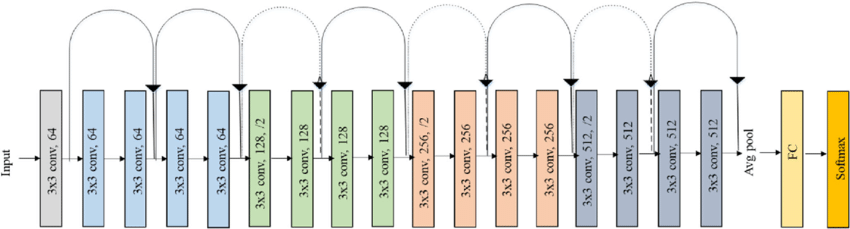
\includegraphics[width=\textwidth]{../../plots/Original-ResNet-18-Architecture.png}
    \caption{ResNet18 Architecture  \cite{deep_learning_alzheimers}}
    \label{fig:resnet18_architecture}
\end{figure}
\textbf{Training Data:} The model is trained on the ASL Alphabet dataset containing 87,000 images resized to 200x200 pixels, spanning 29 classes (26 letters plus 3 additional classes to aid live classification). 10 percent is held out as a test set, so 78,300 images are used in training.
\begin{table}[H]
    \centering
    \caption{Overview of Data Split and Image Specifications}
    \label{tab:datasplit}
    \begin{tabular}{|l|cl|}
    \hline
    \textbf{Category} & \textbf{Number of Images} & \textbf{Percentage} \\
    \hline
    Overall Dataset & 87,000 & 100\% \\
    Training Set & 78,300 & 90\% \\
    \quad Training (90\%) & 62,640 & 72\% \\ 
    \quad Validation (10\%) & 15,660 & 18\% \\ 
    Test Set & 8,700 & 10\% \\
    \hline
    \end{tabular}
    \end{table}
\textbf{Hyperparameters:}
\begin{itemize}
    \item Optimizer: Adam
    \item Loss Function: Cross-Entropy
    \item Learning Rate: 0.01
    \item Batch Size: 64
    \item Epochs: 20 (best validation accuracy selected)
\end{itemize}
\section{Intended Use}
ResNet18 is an instance of the ResNet architecture designed for image classification. Our ResNet18 implementation uses a pre-trained ResNet18 model with transfer learning to classify images of American Sign Language (ASL) letters. The model is intended for:
\begin{itemize}
    \item Classifying American Sign Language alphabet letters from images
    \item Real-time sign language interpretation using live video inputs
\end{itemize}

\section{Performance}
On a separate test dataset, the ResNet18 model achieved:
\begin{itemize}
    \item \textbf{Test Accuracy:} 100\%
    \item \textbf{Precision:} 1.0
    \item \textbf{Recall:} 1.0
\end{itemize}
\begin{figure}[H]
    \centering
    \includegraphics[width=0.8\textwidth]{../../plots/ResNet18_Visualize.png}
    \caption{Feature Maps from the ResNet18 model}
    \label{fig:resnet18_visualize}
\end{figure}
Figure~\ref{fig:resnet18_visualize} shows sample feature maps extracted from intermediate layers of the model.
\begin{figure}[H]
    \centering
    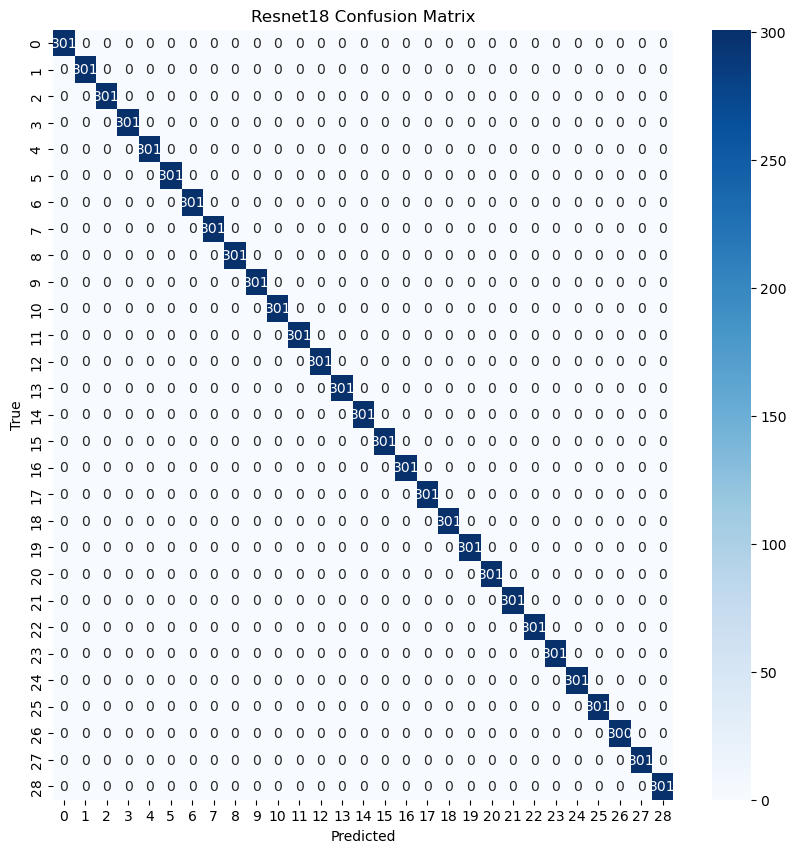
\includegraphics[width=0.8\textwidth]{../../plots/ResNet18_ConfusionMatrix.png}
    \caption{Confusion Matrix for ResNet18}
    \label{fig:resnet18_confusion_matrix}
\end{figure}
\begin{figure}[H]
    \centering
    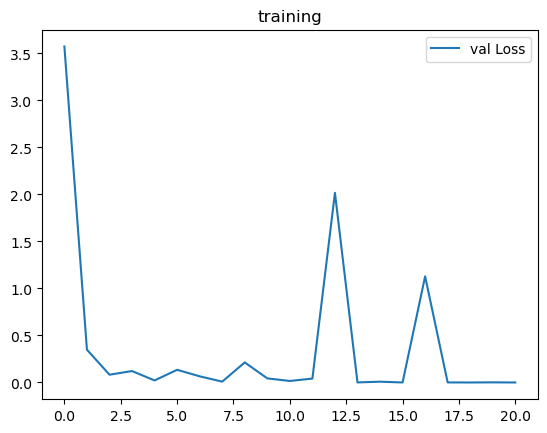
\includegraphics[width=0.8\textwidth]{../../plots/ResNet18_training.png}
    \caption{Training Loss for ResNet18}
    \label{fig:resnet18_training_loss}
\end{figure}


% \begin{figure}[ht]
%     \centering
%     \includegraphics[width=0.7\textwidth]{../plots/ResNet18_Visualize.png}
%     \caption{Feature Maps from ResNet18}
%     \label{fig:resnet18_visualize}
% \end{figure}

\section{Limitations}
Despite high accuracy, some limitations are noted:
\begin{itemize}
    \item Sensitivity to variations in image quality and lighting conditions during live classification
    \item Dependence on precise hand positioning for real-time classification
    \item Potential challenges in deployment on resource-constrained devices
\end{itemize}

\section{Ethical Considerations}
\begin{itemize}
    \item Ensure the ASL dataset is diverse and representative to avoid biased outcomes
    \item Implement privacy protections when deploying real-time video classification
\end{itemize}
\bibliographystyle{IEEEtran}
\bibliography{references}
\end{document}